\begin{align}
    \vec{A} - \vec{B} &=  \myvec{-4\\-1}
    \label{AB}
    \\
    &= -\brak{\vec{C} - \vec{D}}
    \\
\vec{B} - \vec{C} &=
    \myvec{1\\-1}
    \vec{A} - \vec{D} 
    \label{AD}
    \\
    \implies AB \parallel CD,  & BC \parallel AD 
\end{align}
Hence, $ABCD$ is a parallelogram.  Also, 
%
\begin{align}
    \vec{E} &= \frac{\vec{A} + \vec{B}}{2} =   \myvec{1\\\frac{1}{2}}
    \\
    \vec{F} &= \frac{\vec{B} + \vec{C}}{2} =   \myvec{\frac{5}{2}\\\frac{3}{2}}
    \\
    \vec{G} &= \frac{\vec{C} + \vec{D}}{2} = \myvec{0\\\frac{3}{2}}
\\
\vec{H} &= \frac{\vec{A} + \vec{D}}{2} =   \myvec{\frac{-3}{2}\\\frac{1}{2}}
\end{align}\\
and 
\begin{align}
 \frac{\vec{E} + \vec{G}}{2} &=   \myvec{\frac{1}{2}\\1}\\
 & = \frac{\vec{F} + \vec{H}}{2} 
\end{align}
See Fig. \ref{fig;ramsey/1/1/9}.
 \begin{figure}[!ht]
 \centering
 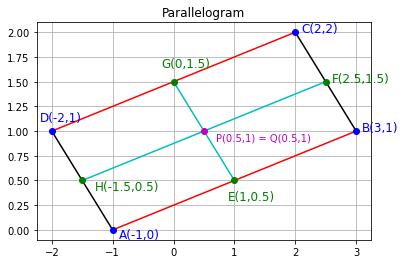
\includegraphics[width=\columnwidth]{solutions/1/1/9/parallelogram.png}
 \caption{}
 \label{fig;ramsey/1/1/9}
 \end{figure}

